\documentclass{report}
\usepackage{graphicx}
\usepackage{color}
\usepackage[colorlinks,urlcolor=blue,linkcolor=black,citecolor=blue]{hyperref}

\begin{document}

\title{Metasploit 3.0 Developer's Guide}
\author{skape}

\begin{titlepage}
    \begin{center}
        \huge{{Metasploit 3.0 Developer's Guide}} \\[150mm]
        \rule{10cm}{1pt} \\[8mm]
        \small\bf{skape} \\
        \small\bf{mmiller@hick.org} \\[4mm]
        \textit{Last modified: \small{11/24/2003}}
    \end{center}
\end{titlepage}

\tableofcontents

\setlength{\parindent}{0pt} \setlength{\parskip}{8pt}

\chapter{Introduction}

\par
The Metasploit framework is an open-source exploitation framework
that is designed to provide security researches and pen-testers with
a uniform model that allows for the rapid development of exploits,
payloads, encoders, NOP generators, and reconnaissance tools.  The
framework provides exploit writers with the ability to re-use large
chunks of code that would otherwise have to be copied or
re-implemented on a per-exploit basis.  To help further this cause,
the Metasploit staff is proud to present the next major evolution of
the exploitation framework: version 3.0.

\par
The 3.0 version of the framework is a re-factoring of the 2.x branch
which has been written entirely in Ruby.  The primary goal of the
3.0 branch is to make the framework easy to use and extend from a
programmatic aspect.  This goal encompasses not only the development
of framework modules, such as exploits, but also to the development
of third party tools and plugins that can be used to increase the
functionality of the entire suite.  By developing an easy to use
framework at a programmatic level, it follows that exploits and
other extensions should be easier to understand and implement than
those provided in earlier versions of the framework.

\par
This document will provide the reader with an explanation of the
design goals, methodologies, and implementation details of the 3.0
version of the framework.  Henceforth, the 3.0 version of the
framework will simply be referred to as \textit{the framework}.

    \section{Why Ruby?}

\par
During the development of the framework, the one recurring question
that the Metasploit staff was continually asked was why Ruby was
selected as the programming language.  To avoid having to answer
this question on an individual basis, the authors have opted for
explaining their reasons in this document.

\par
The Ruby programming language was selected over other choices, such
as python, perl, and C++ for quite a few reasons.  The first, and
primary, reason that Ruby was selected was because it's a language
that the Metasploit staff enjoyed writing in.  After spending time
analyzing other languages and factoring in past experiences, the
Ruby programming language was found to offer both a simple and
powerful approach to an interpreted language.  The degree of
introspection and the object-oriented aspects provided by Ruby was
something that fit very nicely with some of the requirements of the
framework, where automated class construction and for the purpose of
code re-use was a very key concern, and it was one that perl was not
very well suited to offer. On top of this, the syntax is incredibly
simplistic and provides the same level of language features that
other more accepted languages have, like perl.

\par
The second reason Ruby was selected was because of its platform
independent support for threading.  While a number of limitations
have been encountered during the development of the framework under
this model, the Metasploit staff has observed a marked performance
and usability improvement over the 2.x branch.  Future versions of
Ruby (the 1.9 series) will back the existing threading API with
native threads for the operating system the interpreter is compiled
against which will solve a number of existing issues with the
current implementation, such as permitting the use of blocking
operations.  In the meantime, the existing threading model has been
found to be far superior to a forking model, especially on platforms
that lack a native fork implementation like Windows.

\par
Another reason that Ruby was selected was because of the supported
existence of a native interpreter for the Windows platform.  While
perl has a cygwin version and an ActiveState version, both are
plagued by usability problems.  The fact that the Ruby interpreter
can be compiled and executed natively on Windows drastically
improves performance.  Furthermore, the interpreter is also very
small and can be easily modified in the event that there is a bug.

\par
The Python programming language was also a language candidate. The
reason the Metasploit staff opted for Ruby instead of Python was for
a few different reasons.  The primary reason is a general distaste
for some of the syntactical annoyances forced by Python, such as
block-indention.  While many would argue the benefits of such an
approach, some members of the Metasploit staff find it to be an
unnecessary restriction.  Other issues with Python center around
limitations in parent class method calling and backward
compatibility of interpreters.

\par
The C/C++ programming languages were also very seriously considered,
but in the end it was obvious that attempting to deploy a portable
and usable framework in a non-interpreted language was something
that would not be feasible.  Furthermore, the development time-line
for this language selection would most likely be much longer.

\par
Even though the 2.x branch of the framework has been quite
successful, the Metasploit staff encountered a number of limitations
and annoyances with perl's object-oriented programming model, or
lack thereof.  The fact that the perl interpreter is part of the
default install on many distributions is not something that the
Metasploit staff felt was worth detouring the language selection.

\chapter{Architecture and Design}

\par
The framework was designed to be as modular as possible as to
encourage the re-use of code across various projects.  The most
fundamental piece of the architecture is the \textit{Rex} library
which is short for the \texttt{Ruby Extension Library}\footnote{This
library has many similarities to the 2.x Pex library}. Some of the
components provided by Rex are a wrapper socket subsystem,
implementations of protocol clients and servers, a logging
subsystem, exploitation utility classes, and a number of other
useful classes.  Rex itself is designed to have no dependencies
other than what comes with the default Ruby install. In the event
that a Rex class depends on something that is not included in the
default install, the failure to find such a dependency should not
lead to the inability to use Rex.

\par
The framework itself is broken down into a few different pieces, the
most low-level being the \textit{framework core}.  The framework
core is responsible for implementing all of the required interfaces
that allow for interacting with exploit modules, sessions, and
plugins. This core library is extended by the \textit{framework
base} which is designed to provide simpler wrapper routines for
dealing with the framework core as well as providing utility classes
for dealing with different aspects of the framework, such as
serializing module state to different output formats.  Finally, the
base library is extended by the \textit{framework ui} which
implements support for the different types of user interfaces to the
framework itself, such as the command console and the web interface.

\par
Separate from the framework are the modules and plugins that it's
designed to support.  A framework module is defined as being one of
an exploit, payload, encoder, NOP generator, or recon tool. These
modules have a well-defined structure and interface for being loaded
into the framework.  A framework plugin is very loosely defined as
something that extends the functionality of the framework or
augments an existing feature to make it act in a different manner.
Plugins can add new commands to user interfaces, log all network
traffic, or perform whatever other action might be useful.

\par
Figure \ref{fig-arch-pkg} illustrates the framework's inter-package
dependencies.  The following sections will elaborate on each of the
packages described above and the various important subsystems found
within each package.  Full documentation of the classes and APIs
mentioned in this document can be found in the auto-generated API
level documentation found on the Metasploit website.

\begin{figure}[h]
\begin{center}
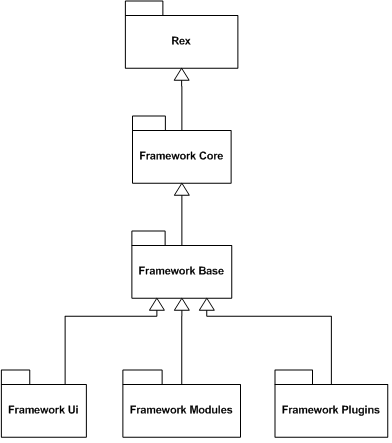
\includegraphics[height=4in,width=4in]{dev_guide_arch_packages}
\caption{Framework 3.0 package dependencies} \label{fig-arch-pkg}
\end{center}
\end{figure}

    \section{Rex}

\par
The \textit{Rex} library is a collection of classes and modules that
may be useful to more than one project.  The most useful classes
provided by the library are documented in the following subsections.

        \subsection{Assembly}

\par
When writing exploits it is often necessary to have to generate
assembly instructions on the fly with variable operands, such as
immediate values, registers, and so on.  To support this
requirement, the Rex library provides classes under the
\texttt{Rex::Arch} namespace that implement architecture-dependent
opcode generation routines as well as other architecture-specific
methods, like integer packing.

            \subsubsection{Integer packing}

\par
Packing an integer depends on the byte-ordering of the target
architecture, whether it be big endian or little endian.  The
\texttt{Rex::Arch.pack\_addr} method supports packing an integer
using the supplied architecture type (\texttt{ARCH\_XXX}) as an
indication of which byte-ordering to use.

            \subsubsection{Stack pointer adjustment}

\par
Some exploits require that the stack pointer be adjusted prior to
the execution of a payload that modifies the stack in order to
prevent corruption of the payload itself.  To support this, the
\texttt{Rex::Arch.adjust\_stack\_pointer} method provides a way to
generate the opcodes that lead to adjusting the stack pointer of a
given architecture by the supplied adjustment value.  The adjustment
value can be positive or negative.

            \subsubsection{Architecture-specific opcode generation}

\par
Each architecture that currently has support for dynamically
generating instruction opcodes has a class under the
\texttt{Rex::Arch} namespace, such as \texttt{Rex::Arch::X86}.  The
x86 class has support for generating \texttt{jmp}, \texttt{call},
\texttt{push}, \texttt{mov}, \texttt{add}, and \texttt{sub}
instructions.

        \subsection{Encoding}

\par
Encoding buffers using algorithms like XOR can sometimes be useful
outside the context of an exploit.  For that reason, the Rex library
provides a basic set of classes that implement different types of
XOR encoders, such as variable length key XOR encoders and additive
feedback XOR encoders.  These classes are used by the framework to
implement different types of basic encoders that can be used by
encoder modules.  The classes for encoding buffers can be found in
the \texttt{Rex::Encoding} namespace.

        \subsection{Exploitation}

\par
Often times vulnerabilities will share a common attack vector or
will require a specific order of operations in order to achieve the
end-goal of code execution.  To assist in that matter, the Rex
library has a set of classes that implement some of the common
necessities that exploits have.

            \subsubsection{Egghunter}

\par
In some cases the exploitation of a vulnerability may be limited by
the amount of payload space that exists in the area of the overflow.
This can sometimes prevent normal methods of exploitation from being
possible due to the inability to fit a standard payload in the
amount of room that is available.  To solve this problem, an exploit
writer can make use of an \textit{egghunting} payload that searches
the target process' address space for an egg that is prefixed to a
larger payload.  This requires that an attacker have the ability to
stick the larger payload somewhere else in memory prior to
exploitation.  In the event that an egghunter is necessary, the
\texttt{Rex::Exploitation::Egghunter} class can be used.

            \subsubsection{SEH record generation}

\par
One attack vector that is particularly common on the Windows
platform is what is referred to as an SEH overwrite.  When this
occurs, an SEH registration record is overwritten on the stack with
user-controlled data.  To leverage this, the handler address of the
registration record is point to an address that will either directly
or indirectly lead to control of execution flow.  To make this work,
most attackers will point the handler address at the location of a
\texttt{pop/pop/ret} instruction set somewhere in the address space.
This action returns four bytes before the location of the handler
address on the stack.  In most cases, attackers will set two of the
four bytes to be equivalent a short jump instruction that hops over
the handler address and into the payload controlled by the attacker.

\par
While the common approach works fine, there is plenty of room for
improvement.  The \texttt{Rex::Exploitation::Seh} class provides
support for generating the normal (static) SEH registration record
via the \texttt{generate\_static\_seh\_record} method.  However, it
also supports the generation of a dynamic registration record that
has a random short jump length and random padding between the end of
the registration record and the actual payload.  This can be used to
make the exploit harder to signature in an IDS environment.  The
generation of a dynamic registration record is provided by
\texttt{generate\_dynamic\_seh\_record}.  Both methods are by the
\texttt{generate\_seh\_record} method that decides which of the two
methods to use based on evasion levels.

        \subsection{Logging}

\par
The Rex library provides support for the basic logging of strings to
arbitrary log sinks, such as a flat file or a database.  The logging
interface is exposed to programmers through a set of
globally-defined methods: \texttt{dlog}, \texttt{ilog},
\texttt{wlog}, \texttt{elog}, and \texttt{rlog}.  These methods
represent debug logging, information logging, warning logging, error
logging, and raw logging respectively.  Each method can be passed a
log message, a log source (the name of the component or package that
the message came from), and a log level which is a number between
zero and three.  Log sources can be registered on the fly by
\texttt{register\_log\_source} and their log level can be set by
\texttt{set\_log\_level}.

\par
The log levels are meant to make it easy to hide verbose log
messages when they are not necessary.  The use of the three log
levels is defined below:

            \subsubsection{LEV\_0 - Default}

This log level is the default log level if none is specified.  It
should be used when a log message should always be displayed when
logging is enabled. Very few log messages should occur at this level
aside from necessary information logging and error/warning logging.
Debug logging at level zero is not advised.

            \subsubsection{LEV\_1 - Extra}

This log level should be used when extra information may be needed
to understand the cause of an error or warning message or to get
debugging information that might give clues as to why something is
happening.  This log level should be used only when information may
be useful to understanding the behavior of something at a basic
level.  This log level should not be used in an exhaustively verbose
fashion.

            \subsubsection{LEV\_2 - Verbose}

This log level should be used when verbose information may be needed
to analyze the behavior of the framework.  This should be the
default log level for all detailed information not falling into
LEV\_0 or LEV\_1. It is recommended that this log level be used by
default if you are unsure.

            \subsubsection{LEV\_3 - Insanity}

This log level should contain very verbose information about the
behavior of the framework, such as detailed information about variable
states at certain phases including, but not limited to, loop iterations,
function calls, and so on.  This log level will rarely be displayed,
but when it is the information provided should make it easy to analyze
any problem.

        \subsection{Post-exploitation}
        \subsection{Protocols}
        \subsection{Services}
        \subsection{Socket}
        \subsection{Synchronization}
    \section{Framework Core}
        \subsection{Event Notifications}
        \subsection{Framework Managers}
    \section{Framework Base}
        \subsection{Configuration}
        \subsection{Logging}
        \subsection{Serialization}
        \subsection{Simplified Framework}
    \section{Framework Ui}
        \subsection{Console}
        \subsection{Web}
\chapter{Framework Modules}
    \section{Encoder}
    \section{Exploit}
        \subsection{Stances}
        \subsection{Types}
        \subsection{Mixins}
    \section{Nop}
    \section{Payload}
        \subsection{Single}
        \subsection{Stage}
        \subsection{Stager}
    \section{Recon}
        \subsection{Discovery}
        \subsection{Analyzer}
\chapter{Framework Plugins}
    \section{User-interface Plugins}
\chapter{Methodologies}
    \section{Writing an Exploit}
\chapter{Conclusion}

\end{document}
